\chapter{Ανίχνευση αντικειμένων χρησιμοποιώντας το νευρωνικό δίκτυο GoogLeNet}\label{ch:googlenet}

In Chapter~\ref{ch:ganeti}, we discussed about Ganeti's architecture; we covered
extensively its most basic components and all the prerequisites needed for
someone to get familiar with this tool. In this chapter, we will discuss how
Ganeti's current design impacts its performance and its scalability, and
then we will provide a design solution for limiting some of those issues and make
the tool even more suitable for cloud environments.

Specifically, section~\ref{sec:obj}, discusses in a few words the current
document's objective and how we are going to succeed it. Section
\ref{sec:back}, provides a detailed view of the configuration and job queue
storage, in addition to the main issues resulting from those design choices. The
options which lead us to the product choice are discussed in section
\ref{sec:cho}, while section \ref{sec:couch} covers in more details the tool
we chose to overcome those performance issues, and more specific the Apache
CouchDB database. Section~\ref{sec:des} finally, provides a detailed
presentation of our software design.

\section{Objective}\label{sec:obj}

Ganeti has been evolved since first introduced, and has become a mature software
tool for managing the low level VM of big clusters. In version 2.7, many new
features like the opportunistic locking where introduced, but many scalability
and performance issues are still arise from the current design.

In the current chapter, we will introduce a different approach for handling the
Ganeti's configuration and job queue storage, using a NoSQL database as the
backend storage layer, which will attempt to remedy some of the performance and
scalability issues that exist in Ganeti version 2.7.

\section{Background}\label{sec:back}

While Ganeti v2.7 is usable, it limits the flexibility and the performance of
the cluster. The current design for handling the configuration data and the job
queue storage, in addition to how it replicates those files among the master
candidate nodes, are some of the main reasons of those limitations. In the
current section we will analyze this design, and we will extensively discuss
about the main issues arisen from it.

More specifically, Section~\ref{sec:config} presents analytically the
configuration data form, in more details than the previous chapter, while
section~\ref{sec:queue}, concentrates on the job storage.
Section~\ref{sec:caveats}, points out the most important performance issues
that arise from the current design, both for the configuration file and the job
queue storage.

\subsection{Cluster configuration data}\label{sec:config}

In section~\ref{sec:architecture}, we saw that the Ganeti's cluster
configuration database is stored in a single file, the \texttt{config.data}
file, on the master node filesystem. In this section, we will dive into the
internal structure of the \texttt{config.data} file, which will lead us to the
conjecture that the current configuration management is imperfect and suffers
from scalability problems mainly on bigger clusters.

The configuration data uses JSON format, consisting of key/value pairs.
The keys that the configuration file consists of, are a combination of Ganeti
specific object collections, and default JSON objects of name/value pairs.
In detail, there are five Ganeti objects namely: \texttt{Cluster},
\texttt{Node}, \texttt{Instance}, \texttt{Nodegroup}, and
\texttt{Network}. From these objects the \texttt{cluster}, \texttt{nodes},
\texttt{instances}, \texttt{nodegroups}, and \texttt{networks} attributes are
composed of. The default name/value pairs are the \texttt{serial\_no},
\texttt{version}, \texttt{ctime}, and \texttt{mtime}. Ganeti configuration
objects provide the appropriate functions for serializing, de-serializing, and
handling them in a safe way, in order to by easily handled by external parties.
They also provide recursive checks for their derived classes, and are also
responsible for handling appropriately any attribute error that will arise.

The configuration file is represented internally by a \texttt{ConfigData}
object, which actually is the topmost-level configuration object.
The \texttt{cluster} attribute contains all the available information that
the cluster needs to operate normally like the master node name, the master ip,
the default hypervisor chosen during cluster initialization, the
candidate\_pool\_size, and more. The \texttt{nodes} attribute, contains all the
nodes that the cluster consists of. Each distinct \texttt{Node} object, contains
information about the corresponding node such as its name, its primary and
secondary IP, the node role information, and more. The \texttt{instances},
\texttt{nodegroups}, and \texttt{networks} attributes, contain relevant
information for the instances that the cluster contains, the nodegroups which
the user created, and the networks that exist in the cluster, as their names
denote.

Besides the Ganeti specific objects, \texttt{config.data} also contains
information about four general attributes. That are, the \texttt{serial\_no},
which is an increasing number denoting the number that the \texttt{config.data}
has been modified since it has been created, and it is used for
consistency checks in case when some candidates are stalled in the middle of a
configuration update, or in order to find the most recent answer when used by
the configuration daemon ,i.e., \texttt{confd}. The \texttt{version} attribute,
contains the current Ganeti version, and the \texttt{\{c/m\}time} timestamps
contain the exact time when the cluster was created and modified, respectively.

Listing~\ref{lst:config}, briefly presents the \texttt{config.data} internal
structure with its most basic key/value pairs. Due to its size, most of its
attributes and values have been intentionally removed for simplicity reasons.

\newpage
\includeminted[text]{../listings/config_data.json}{%
  Structure of the \texttt{config.data} file}{lst:config}{linenos}

\subsection{Job storage}\label{sec:queue}

Jobs are stored in the filesystem as separate, individual files using JSON
format just like the \texttt{config.data} file. The choice of storing each job
in its own separate file was made for a number of reasons. The most important of
them are summarized below.

In chapter~\ref{ch:ganeti}, we saw that a job can change its status many times
during its execution ,e.g., Queued, Waiting, Running, and more. Moreover, an
opcode, so as the job, passes from several execution phases like acquiring
the needed locks, running the iallocator algorithm, and so on. The user should
have access to all that information when requests it, either for debugging
reasons, or simply for monitoring the execution path of a job. Those information
is saved in the job object as a list of log messages in the \texttt{log}
attribute. It is obvious that a job is modified many times during its execution.
The choice of using a file per job, is based on the fact
that a job changes quite often, and a file that can easily and atomically be
(over)written facilitates this behavior. Furthermore, a file can be easily
replicated to the master candidate nodes. The replication is done atomically for
every single file with a multi-node \texttt{Remote Procedure Call (RPC)} call
with a timeout of about a minute. In addition, a consistency check in the job
queue across master candidate nodes through a third partie, can very easily be
implemented, since all job files should be identical.

It is also interesting to see how a job is internally represented by Ganeti.
Jobs are stored in the filesystem, but until the job completes its execution
there is also an in-memory representation of it. Any modification to the job
object is flushed on the disk, and then replicated to the candidate nodes. That
in-memory representation of a job is a python class definition called
\texttt{\_QueuedJob}. This class contains attributes and implements all the
appropriate methods needed for the smooth execution of a job. The most important
attributes that a \texttt{\_QueuedJob} object contains are: the job \texttt{id}
field, the \texttt{queue} object on which the job belongs, the \texttt{ops}
field which is a list of the job's opcodes where the \texttt{\_QueuedOpCodes}
objects are encapsulated, and three timestamps the \texttt{received},
\texttt{start}, and \texttt{end}, providing information about the time when a
job was received, started and finished its execution respectively.

\subsection{Caveats}\label{sec:caveats}

We extensively discussed about the design of Ganeti. While it scales quite well
for small clusters, it does not as the number of nodes grow, and some drawbacks
start to appear. This is mainly due to the fact that several documents are
shared among the nodes of the cluster. The \texttt{config.data} file and the job
queue need to be present, and replicated, to all master candidates for
reliability reasons mainly, and the \texttt{ssconf\_} static configuration
files have to be replicated to all the nodes of the cluster, as well. In
addition, the \texttt{confd} which is present on all the master candidate nodes,
might need to have access to the configuration data file even if the master node
is down. Due to those needs, an increase in the size of the cluster will bring
up the configuration management imperfections that Ganeti suffers of. In
particular:


\begin{itemize}
  \item Some operations like \texttt{instance-(add/remove/rename)},
        \texttt{network-(add/remove)}, or
        \texttt{node-(add/remove/offline/drained)} are the most commonly used
        operations in a Ganeti cluster. Some of these operations like the
        instance related ones, grow in frequency as the cluster grows. We would
        ideally want the  time needed in order to those operations to complete,
        be steady. This does not apply at all, due to the fact that all these
        operations need to contact all the nodes of the cluster in order to
        update the \texttt{ssconf\_} files, so they become significantly slower.
  \item Any other operations that do not affect the \texttt{ssconf\_} files
        will contact, at least, all the master candidate nodes for two reasons.
        The first one is to inform the configuration data files for the new
        updates been made, and the second one is to synchronize the job queues
        among them. As the number of nodes in a cluster grows, we expect the
        number of jobs to grow as well. While the number of candidate nodes is
        constant, an increase on the jobs will have impact on the cluster
        performance. This is due to the fact of an overloaded master daemon
        which will affect the whole cluster performance, because besides the
        growth in the number of jobs it has to deal with, it also has to
        supervise the replication process of those files among the candidate
        nodes, manage the locking, an so on.
  \item The candidate pool size is not affected as the cluster size
        increases. It is a constant number independent of the nodes of the
        cluster. Ganeti though, interacts with the candidate nodes every time
        it updates one of its configuration and job queue files in order to
        maintain the file consistency among them. The replication procedure is
        the main reason that prevents Ganeti from scaling. It is handled and
        monitored exclusively by the master daemon, and is a procedure that
        breaks the scalability because many should-be-fast operations are slowed
        down by replicating the changes to remote nodes, thus waiting with locks
        held on remote RPC calls to complete.
  \item Another issue arisen from the increase in the number of jobs, is the
        \emph{config lock}. Any job that modifies the cluster state must
        exclusively acquire that lock before apply its changes to the cluster,
        and so as to the configuration file. The single config lock becomes a
        bottleneck, when a huge number of jobs is in execution and try to
        acquire it. In addition, the lock will not be released until the
        modification have been successfully replicated to the master candidate
        nodes, something that increases the congestion on that lock.
  \item The configuration file is a JSON formatted file which needs to be
        serialized before it is flushed to disk. The time needed to serialize
        it, is quite small in smaller clusters and it can be ignored. Ganeti
        though, is a tool used by big open source projects, such as Synnefo
        \flink{http://www.synnefo.org}, which means it is mainly used in bigger
        clusters. Providing an example, a cluster with around \emph{1.000}
        instances, will have a \texttt{config.data} file of about \emph{2.5 MB}
        in size. The serialization cost starts to be a bottleneck when the
        configuration file enlarges, even from sizes at around \emph{1 MB}. This
        claim will be justified in Chapter~\ref{ch:performance}. The
        de-serialization cost from disk is also raised respectively, but it does
        not affect the overall cluster performance at all, because the
        \texttt{config.data} de-serializes only at the master-daemon startup.
        Then it exists at the master node memory, and its disk version is
        updated from there.
  \item Besides the serialization cost, more factors are affected when the
        configuration data size increases. These are the time needed to
        flush the changes to disk, in addition to the time needed to distribute
        those modifications to the master candidates. These two extra costs, in
        addition to the serialization time discussed in the bullet above, slows
        down the cluster operations, reduce the overall performance of the
        cluster and make even the quick commands last several minutes,
        instead of some seconds in order to complete.
  \item The current configuration management groups all the cluster's attributes
        in a single JSON file ,e.g., instances, nodes, networks, and more. This
        design choice, in combination to the global config lock, forbids any
        type of concurrent update to distinct Ganeti objects, and makes every
        modification access to the configuration file be serialized. There are
        various cases when that restriction reduces the cluster performance. An
        example is when a client wants to add an instance to the cluster, while
        another one tries to create a new network. While the clients modify two
        distinct objects of the cluster with an indirect
        relationship, they can not make the updates concurrently, but they have
        to wait instead. It would be very convenient for Ganeti and its users to
        allow concurrent updates when they do not affect other cluster
        operations, because it would have a positive impact in the cluster's
        throughput.
  \item Moreover, in case of a faulty update on the configuration file, there is
        no way to roll back the changes made in it and return to a previous
        state. Even if we keep backups of the configuration file and want to
        revert a modification, we should alter the whole configuration file and
        not only the section that we modified, increasing the probability of
        causing a breakage in the cluster configuration state. This attribute
        could be very useful in case when the \texttt{config.data} breaks due to
        a faulty-update on it, and we want to recover it painless.
\end{itemize}

\section{Choice of product}\label{sec:cho}

Our design solution aims to address some, and not all, of the above issues.
It replaces the Ganeti configuration and job queue storage with a NoSQL
distributed, document-oriented database. There are plenty of NoSQL choices in
the database market which would meet Ganeti's requirements, such as MongoDB
\flink{http://www.mongodb.org/}, or Riak~\flink{http://basho.com/riak/}. Some of
the criteria for deciding which one was the best fitted NoSQL solution for
Ganeti were the replication style, the reliability provided, the available API,
and how the database handles reads and writes. For our implementation we chose
\emph{Apache CouchDB}~\flink{http://couchdb.apache.org/} as our backend
database.

Apache CouchDB (acronym of \emph{``Cluster Of Unreliable Commodity Hardware"}),
is an open source database built on the Erlang OTP platform~\flink{http://www.
erlang.org}, a functional, concurrent programming language, and a development
platform too. Erlang was developed for real-time telecom applications with an
extreme emphasis on reliability and availability using lightweight ``processes"
and message passing for concurrency. It is an
ideal solution for a database server due to its robustness and concurrent
nature. CouchDB is a database that focuses on being \emph{``a database that
completely embraces the web"}, as its developers promote. It is a NoSQL
document-oriented database, using JSON format for storing its data, a simple
RESTful API based on HTTP, and a powerful query server using Map/Reduce
techniques that is written in JavaScript, by default, but there are also servers
available for nearly any language we can
imagine~\flink{http://en.wikipedia.org/wiki/CouchDB}.
It was created in April 2005 by Damien Katz, and since February 2008 is part of
the Apache foundation. In July 2013, the CouchDB community merged the codebase
for BigCouch, Cloudant's clustered version of CouchDB, into the Apache project.
The BigCouch clustering framework is prepared to be included in an upcoming
release of Apache CouchDB~\cite{bigcouch}.

The main reasons we chose CouchDB for our modifications to Ganeti,
are presented in the current section.  We do not claim it is the best fitted
database solution for Ganeti or the only one, but without lost of generality it
is a representative NoSQL database which will show us how Ganeti reacts with a
different underlying storage solution. The criteria which were evaluated are the
following:

\begin{itemize}
  \item \underline{\emph{Free Software,}} CouchDB is an open source project
    which keeps up with the current open source Ganeti policy.
  \item \underline{\emph{Licensing,}} CouchDB is licensed under the Apache
    License, Version 2.0~\flink{http://www.apache.org/licenses/LICENSE-2.0}
    which does not affect Ganeti's license or model. Ganeti will remain a
    separate software, which connects through Apache licensed libraries to
    CouchDB.
  \item \underline{\emph{Bindings,}} Ganeti is written in both python and
    Haskell languages. CouchDB provides Haskell bindings which are available on
    Hackage, the Haskell package library, and a variety of Python libraries for
    working with CouchDB.
  \item \underline{\emph{Document Storage,}} In order to avoid big changes in
    the current configuration and job queue storage we want a solution that
    would fit this design. CouchDB stores its data as documents; one or more
    key/value pairs using JSON format, that fits the Ganeti's needs.
  \item \underline{\emph{Replication model,}} CouchDB is a peer-based distributed
    database system. Its replication process synchronizes two copies of the same
    database. If you change one document of a database, the replication process
    will propagate these changes to the second database.
    This is very similar to the master-slave
    replication procedure used by Ganeti. In addition, the BigCouch merge in the
    CouchDB project will give us a native clustering support which could later
    provide different design solutions for the Ganeti data handling.
  \item \underline{\emph{Simplicity,}} CouchDB comes with good documentation in
    the form of books, presentations, blog posts, wikis, and a strong and active
    community which makes it much simple to be installed and configured. In
    addition, the RESTful HTTP API which uses, is quite straightforward and
    simple, and it does not requires much effort to learn using it.
  \item \underline{\emph{Security model,}} CouchDB comes with a simple reader
    access and update validation model to protect who can read and update
    documents, that can also be extended to support custom security models. In
    addition, every CouchDB database instance can have one or more administrator
    accounts. These accounts come with specific privileges and user credentials
    in order to secure the access to selected databases and documents.
    Validation functions are written in JavaScript, and can be used as documents
    are written to disk. If the documents pass the validation criteria, the
    update is allowed to continue, otherwise the update is aborted and an error
    message is returned to the client.
  \item \underline{\emph{Resource Usage,}} CouchDB is designed from the ground
    up to service highly-concurrent use cases. There is not fixed RAM, CPU or
    disk space needs for CouchDB. It is flexible enough to run from a smart
    phone to a cluster. Apparently, more RAM is better, because CouchDB works
    completely through file I/O, delegating caching to the operating system,
    the filesystem cache. CouchDB makes the assumption that disk space is
    cheap, so it does not take great care of it. The good news are that some
    operations like database \emph{compaction} reclaim a lot of disk space.
    CouchDB is  written in Erlang, so the more CPU in a server, the most
    \emph{beam} processes~\flink{http://www.erlang.org/documentation/doc-5.8.3/
    doc/efficiency\_guide/processes.html} can be created. CouchDB (or Erlang)
    take great advantage of this resource. Summing up, memory and disk have the
    great ``pain", as a result faster disks and more memory will be handy and
    will increase the database overall performance.
  \item \underline{\emph{Debugging,}} CouchDB maintains a log file where every
    single operation, or event made to the CouchDB server is
    recorded. The debugging level of the log file can be modified,
    and the user can define how verbose and detailed the logging will be. We can
    choose from a very informative log file, where every HTTP header, external
    process communications, authorization operations, and much more information
    is recorded, to a status where any debug message is disabled. Ganeti also
    maintains a set of log files to record its updates, and CouchDB will just
    insert one more log file to the already existent.
  \item \underline{\emph{Reliability,}} CouchDB comes with a fault-tolerant
    storage engine that puts the safety of the data first. As it name denotes,
    is build for Clustering On Unreliable Commodity Hardware and the main goal
    is to provide data integrity, high-scalability and reliability in a
    fault-prone environment. The fact that CouchDB is written in Erlang, a
    concurrent, functional programming language with an emphasis on
    fault-tolerance reinforces the succeed of the data safety goal. Its internal
    structure is fault-tolerant, and failures occur in a controlled environment
    and are dealt without letting single problems cascade to the whole system,
    but are isolated in single requests. For CouchDB specifically, if an
    operation fails, we will never end up in a state with partially updated
    objects, or corrupted objects that was previously written successfully to
    the server. It provides a total reliable storage engine, which we will
    extensively present in section~\ref{sec:couch}.
  \item \underline{\emph{Recovery from failures,}} The current CouchDB design
    does not provide automate recovery from failures. The recovery procedure
    will be handled by Ganeti with the administrator help, as it currently is.
    Various commands like the \texttt{master-failover}, or the
    \texttt{redist-conf} will be extended to meet up with the new needs. The
    CouchDB replication procedure, along with the CouchDB tools, will make
    those operations relatively painless.
  \item \underline{\emph{Backups,}} CouchDB stores each database in a separate
    file in the disk, as we are extensively cover in later sections. We can take
    backups of a database file, silently and without stopping the database by
    simply running a \texttt{cp} Unix command ,i.e., \texttt{cp db.couch
    /mnt/backup}. We can store periodically flat-file copies of the database
    files on the master and master candidate nodes, and create a method to
    ``re-init" the Ganeti status from those flat-files during disaster-recovery.
  \item \underline{\emph{Backwards compatibility,}} We would like to have a way
    to easily converting from the current Ganeti storage management, to CouchDB.
    We decided to support both CouchDB and file configuration as different
    storage engines, with different limitations for each case. Maybe it is not
    the simplest solution since it requires to convert a fairly great amount of
    code, but the future ability of further expanding the underlying storage
    options is a tradeoff that reinforces that approach.
\end{itemize}

\section{Apache CouchDB}\label{sec:couch}

In the previous section, we mentioned the factors why we chose CouchDB for our
implementation, depending on current Ganeti needs, keeping also in mind that we
do not want a choice that will introduce important Ganeti design changes. In the
current section we will discuss extensively about Apache CouchDB and its main
characteristics and features, in order to proceed with the detailed design
section.

CouchDB is a document-oriented, distributed, schema-free NoSQL database, using
views for aggregating and reporting on documents in a database. For a complete
overview of CouchDB's technical information there is a well structured
documentation~\flink{http://kxepal.iriscouch.com/docs/dev/contents.html}. Let's
review some of the basic elements of CouchDB:

\begin{description}
  \item[Schema-Free] \hfill \\
    Unlike SQL databases which are designed to support highly-structured data,
    with CouchDB no schema is required. New document types can be added at
    will, alongside with the old ones. CouchDB is designed to perform on
    document-oriented applications with large amounts of semi-structured data.
  \item[Document-Oriented] \hfill \\
    Documents are the primary unit of data in CouchDB. Each document is a JSON
    formatted object and consists of any number of named fields and attachments
    \footnote{Documents in CouchDB can have attachments just like an email. For
    creating an attachment, we need to provide a file name, the MIME type and
    the base64 encoded binary data. Its even possible to have multiple
    attachments for a single document.}.
    Field values can be strings, numbers, dates, or even ordered lists and
    associative arrays. Documents also include metadata that are maintained and
    used by the CouchDB server. An example of a document in CouchDB would be a
    contact document as shown in Listing~\ref{lst:couch_doc}. In that document,
    ``Type" is a field that contains a single string value ``Contact", ``Email"
    is a field containing a list of two values and so on.

    A CouchDB database is a flat collection of documents, each having a unique
    identifier named \texttt{\_id}, and a revision/version number named
    \texttt{\_rev}. The version number is a special field in CouchDB with great
    importance, about which we will talk later in this chapter. The underlying
    data structure used to store the database files is a B+tree structure.
    CouchDB implementation is a bit different from the original B+trees; while
    it maintains all the important properties, it adds an append-only design
    \flink{http://guide.couchdb.org/editions/1/en/btree.html}, along with a
    \emph{Multi-Version Concurrency Control}. That append-only variation of the
    original B+tree structure, trades a bit of (disk) space for speed. A B+tree
    is an excellent data structure for storing huge amount of data for fast
    retrieval. The B+trees are very shallow but wide data structures. The leaf
    nodes contain the actual data in an ordered manner, while the intermediate
    nodes contain indexes/pointers to the nodes beneath them. While
    other tree structures can grow very high, a typical B+tree has a
    single-digit height, even on millions of entries. \emph{Jan Lenhard}, one of
    the core CouchDB developers, said during the \emph{Berlin's Buzzwords 2013}
    conference~\footnote{Berlin Buzzwords is a Germany's conference that
    focuses on the issues of scalable search, data-analysis in the cloud and
    NoSQL-databases} that a B+tree node in CouchDB has a size of about
    \emph{60.000} entries. That actually means that even on billions of entries
    in a database, we will have a tree depth of 6, at most. This is very
    interesting for CouchDB particularly, where the leaves nodes of the B+tree
    are stored in a slow medium such as a hard drive. CouchDB does not make use
    of a built-in cache layer, but it uses the operating system's cache instead.
    Due to the small height of the structure, the filesystem cache keeps the
    upper nodes of the tree cached, so reading, or writing to a document
    requiring only a few seeks to disk on the final tree node, making it a quite
    fast data structure for both read and write requests.

    \includeminted[text]{../listings/couch_doc.json}{%
      Document sample in CouchDB}{lst:couch_doc}{linenos}

  \item[Views] \hfill \\
    CouchDB is a schema-less database. However, for some
    applications a kind of structured data may be required. In order to deal
    with that problem, CouchDB integrates a view model using JavaScript for the
    view description. Views are also a useful tool for many other purposes like
    document filtering based on specific fields, extracting and presenting data
    in a special order, building indexes among documents to find a value that
    resides in them, and generally performing all sorts of calculations on the
    databases data.

    CouchDB views are stored inside special \emph{design documents}, and a design
    document can contain any number of views. A view is actually a map function
    of a map/reduce system. All map functions have a single parameter
    \texttt{doc}, which corresponds to a single document in the database. A simple
    view example which checks whether the database's documents have a date and a
    title field is shown in Listing~\ref{lst:view}. When we query the view,
    CouchDB takes the source code and runs it on every document in the database
    our view was defined. We query the view to retrieve the view result. Because
    the view runs on all documents of a database, it would take a lot amount of
    time to run it, if it should traverse the whole database every time we
    query it. Instead, a view runs on all documents only the first time it is
    queried; if a document is updated the map function will only run to
    recompute the new keys and values for the updated document. Views in CouchDB
    are stored in separate flat files just like the databases, using B+tree data
    structure as well. Initially, the view file is empty because no index has
    been built yet. Views are being built \emph{lazily} when the first query is
    made. The next view query will incrementally update the not updated view
    indexes.

    \includeminted[text]{../listings/view.txt}{%
      View function in Javascript in CouchDB}{lst:view}{linenos}

  \item[ACID properties] \hfill \\
    CouchDB is a database, so every transaction should ensure the ACID
    (Atomicity,  Consistency, Isolation, Durability) properties. CouchDB
    provides ACID semantics, and in this part we will examine carefully each of
    those properties.

    \begin{itemize}
      \item \emph{Atomicity}, refers to the ability of database to guarantee
      that either all the tasks of a transaction are performed or none of them
      are. Each transaction is said to be atomic in case when one part of a
      transaction fails, the whole transaction fails. CouchDB database
      modifications follow the ``all or nothing" rule, ensuring that property.
      \item \emph{Consistency}, is the property that ensures that any
      transaction will bring the database from one valid state to another,
      according to some defined rules. The valid state does not necessarily
      guarantee correctness of the transaction in all ways the application
      programmer might have wanted, but that the database will remain consistent
      even if the transaction succeeds, or fails. For distributed systems, as
      CouchDB is, the system is either strongly consistent or has some form of
      weak consistency, also referred as eventual consistency. CouchDB is an
      eventual consistent database, ensuring that the database will eventually
      reach at a consistent state. The \emph{MVCC} method ensures that each
      client sees a consistent snapshot of the database from the beginning to
      the end of the read operation. The latest version is sitting somewhere in
      the cluster. Older versions are still out there and eventually all nodes
      will see the latest version.
      \item \emph{Isolation}, refers to the requirement that other operations
      cannot access or see the data in an intermediate state during a
      transaction. This constraint is required to maintain the performance as
      well as the consistency between transactions in a database. Thus, each
      transaction is unaware of another transactions executed concurrently in
      the system. It ensures that the concurrent execution of transactions
      results in a system state that would be obtained if transactions were
      executed serially. Documents updates in CouchDB (create, delete, modify)
      are always serialized on disk. In addition, the concurrent update of the
      same document will result in two new documents, where none of the clients
      that modify the same document is aware of the other client existence.
      \item \emph{Durability}, refers to the guarantee that once the user has
      been notified of success, the transaction will persist, and will
      not be undone.
      This means it will survive system failure, and that the database system
      has checked the integrity constraints and will not need to abort the
      transaction. CouchDB uses by default the \emph{fsync} system call, to
      ensure that a transaction have reached the disk before declaring it as
      successful. It also gives the ability to the user to loose that property
      and increase the write performance by using intermediate buffers, but by
      default it always ``fsyncs" for every transaction. In addition, another
      transaction will never overwrite any changes made by a previously
      successful transaction, due to the append-only model followed. So, it
      cannot corrupt anything that has been written and committed to disk
      already.
    \end{itemize}

    In order to understand even better how CouchDB ensures the above properties,
    we are going to give an overview of some more technical, but important,
    CouchDB features:

    CouchDB implements a form of \emph{Multi-Version Concurrency Control (MVCC)}
    \flink{http://en.wikipedia.org/wiki/Multiversion\_concurrency\_control},
    instead of locks. Requests are run in parallel, making excellent use of the
    CPU, but writes are always serialized on disk. Database readers will never
    have to wait for writers or other readers on the same document. Each reader
    sees a consistent snapshot of the database from the beginning till the end
    of the operation. We mentioned earlier that every document always contains
    besides the \texttt{\_id} field, a \texttt{\_rev} field as well. This is the
    document's version, because in CouchDB documents are versioned. If we want to
    modify a document, we create an entire new version of it and save
    it after the old one. So, we end up with more than one versions of the same
    document, depending on how many times we modify it. The version is a
    composition of two values ,i.e., \texttt{``23-a2a33fdabad1376f58a12ea0ff4b"}.
    The first one is an increasing sequential number, which denotes how many
    times the file was modified. The second part of the number after the dash,
    is a hash composition of the document's contents plus the sequential number
    of the revision. If we found two documents, in different databases, with
    same \texttt{\_id} and \texttt{\_rev} values its not necessary to look at the
    contents of each file to know that are identical, we already know they are.
    In that lockless update model we may end up with two clients updating the
    same document. In that case, a  conflict error will be produced, where two
    versions of the same document will exist. There is a conflict mechanism used
    by CouchDB to resolve those errors, and the user can also involve in the
    conflict resolution. There are three possible states after a conflict
    detection, which are explained in the \texttt{Eventual Consistency} section
    \ref{item:eventual}, and ensure that the database remains consistent even if
    sometimes the application should involve in that procedure.

    \emph{Committing} is the process of updating the database file to reflect
    the changes requested. It is a CouchDB process with great importance. It is
    not needed in order to use CouchDB, but it will help us to deeper understand
    the CouchDB design, and how the ACID properties are preserved. CouchDB uses a
    B+tree data structure for both the ``storage" and the ``view" needs. In that
    paragraph we will focus on the storage part. Every database file consists
    internally of a number of components. The most important of them follow:

    \begin{itemize}
      \item \emph{B+tree, by\_id\_index}. It is a B+tree structure that uses the
      document ID as the index key. This index stores the mapping from document
      IDs to their positions on disk. Is is mainly used to lookup documents by
      their ID. The data on disk it points to, contain the list of revisions,
      along with the document's revision history.
      \item \emph{B+tree, by\_seqnum\_index}. It is a B+tree structure that uses
      the sequence number as the index key. A new sequence number is a
      monotonically increasing number, and is generated every time a document is
      created, deleted, or modified. This index stores the mapping from the
      update sequence number to the document's position on disk. This B+tree
      actually answers the question \emph{``what happened since?"}, and is very
      useful to keep track of the last point of the replication synchronization
      or the last point of view index updates, by the \emph{compaction}
      operation, and more.
      \item \emph{Header}. The file header contains the pointer to the roots of
      the above two B+tree structures, some metadata needed by the CouchDB
      server like the database name, or size, and a checksum to ensure the
      file's integrity.
    \end{itemize}

    CouchDB database files are purely append-only. This means that all document
    updates like create, delete, and modify happen in a purely append-only
    mechanism. All writes occur at the end of the file, and old versions of
    documents are never overwritten, or deleted when new versions come in. Either
    inserting or deleting a document, the database file still grows only at the
    end. More specifically, CouchDB uses a kind of copy-on-modified approach.
    This means that the update is not happening in-place, but after we located
    the B+tree node that contains the document to be modified, we copy it over,
    make the appropriate modifications, and append it at the end of the file.
    After that, the parent B+tree nodes should also be informed to point to the
    new location. A modification to the parent node is triggered, which will
    also cause a new copy of the parent node, and so on all the way back to the
    root node of the B+tree. Finally, the file header must be modified to point
    to the new root node location. That means that every update will trigger 1
    write to the document and \emph{logN} writes to the B+tree nodes, where N is
    the B+tree height. A graphical representation of this procedure from a
    high-level of view is shown in Figure~\ref{fig:btree}, which was taken from
    a blog post by Ricky Ho titled, ``NoSQL patterns"
    \flink{http://horicky.blogspot.gr/2009/11/nosql-patterns.html}. Notice that
    the update of a data slot causes the creation of the \emph{green} nodes,
    while the \emph{yellow} ones will be removed as soon as no one uses them,
    after a compaction operation.

    \begin{figure}[htbp]
      \begin{center}
        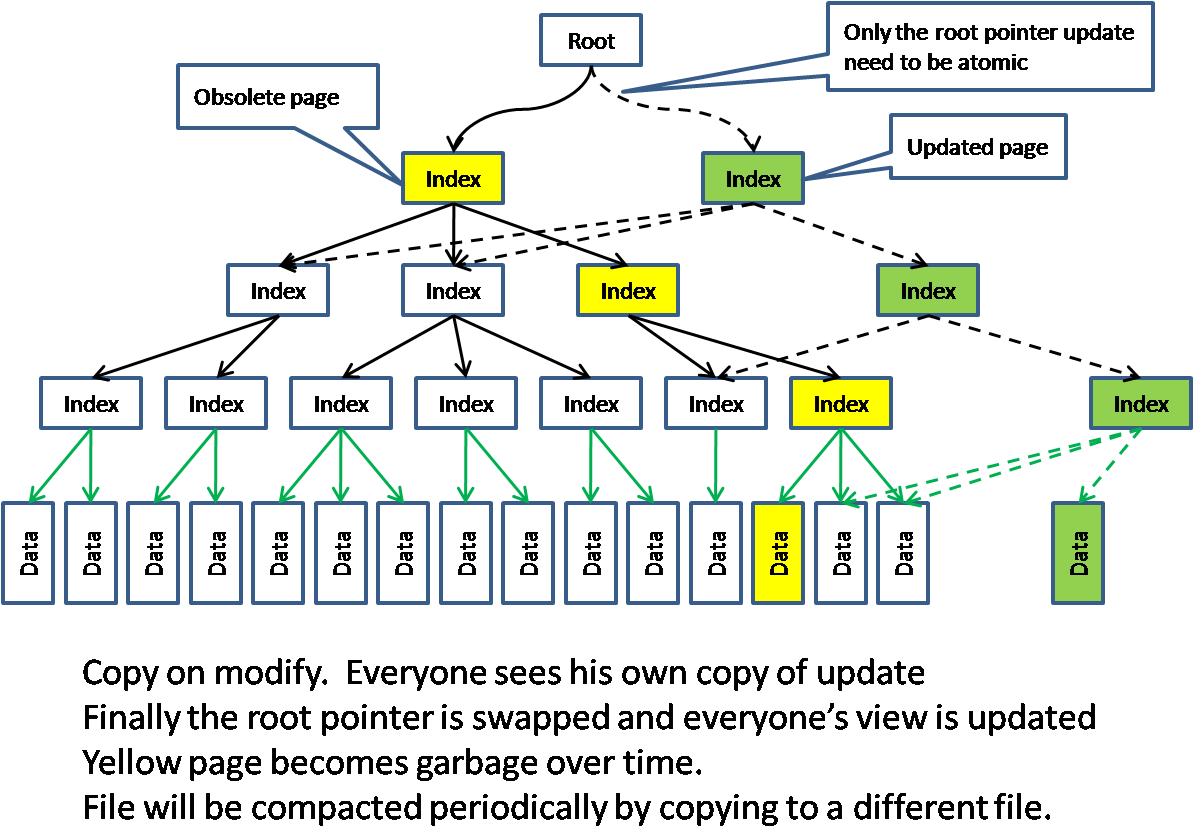
\includegraphics[width=0.9\maxwidth]{../figures/b-tree.pdf}
        \caption{The power of B+trees in CouchDB\label{fig:btree}}
       \end{center}
    \end{figure}

    The update mechanism also forbids partial updates; either the update will
    succeed or will fail completely, there is nothing in between. The file
    footer is the last region that is updated and appended at the end of the file
    during a transaction. It is the last 4K of the database file, and is actually
    the database header we explained above. To declare an operation successful
    the footer must be written twice. It is separated in two identical chunks
    of 2K each. The committing process occurs in two phases. During the first
    phase, CouchDB appends any changes in terms of document data and their
    associated indexes to the file. After recorded the new file's length, it
    records it to the first 2K of the file footer. Those updates are
    synchronously flushed to disk. In the second phase it just copies the first
    2K of the footer, over the second 2K of the footer, and flushes again. Only
    when both footers are flushed to disk CouchDB declares the transaction as
    successful. If a failure happens during phase 1, the partially flushed
    updates are simply forgotten. Incomplete writes and index updates simply
    appear as garbage data at the end of the file, and are ignored on database
    open. If a failure happens during the header committing (phase 2), CouchDB
    start reading the file backwards~\footnote{To differentiate data from
    headers, CouchDB appends a single byte every 4K of the database file. If the
    byte value is 0x01, everything preceding is database header. If the value is
    0x00 then document data precedes.}. If the first 2K is corrupted, CouchDB
    replaces it with the second identical 2K footer. The same happens if the
    second 2K are corrupted. If the header is intact then the data are intact as
    well. Checks never happen in the document data or their associated indexes,
    but only in the database header. With this design data are never lost, and
    data on disk are never corrupted.

    This append-only design results in very fast updates, and query processing.
    Provided that the B+tree nodes are in system memory, they require the
    minimal seeks possible. A tradeoff of this scheme is the disk space needs.
    CouchDB is built with the assumption of cheap disk space, but since every
    document update causes a whole new copy of the B+tree indexes, care should
    be taken for limiting the disk space needs. CouchDB answer is the
    \emph{compaction} operation. Compaction compresses the database file by
    removing unused sections created during updates. Old revisions of documents
    are also removed from the database, though a small amount of meta data is
    kept for server related needs. It is manually triggered per
    database and retrieves a great amount of disk space. Technically, the
    compaction process opens the file and reads the \emph{by\_seqnum\_index}.
    It traces the B+tree all the way to the leaf node and
    copy the corresponding document content to the new file. The database
    remains completely online the entire time and all updates and reads are
    allowed to complete successfully. The old file is deleted only when all the
    data has been copied and all users transitioned to the new file.
  \newpage
  \item[Distributed Updates and Replication]\label{item:replication} \hfill \\
    Maybe the most powerful CouchDB's feature is the simplicity of replicating
    databases among different servers in the web. Replication is an incremental,
    fast, and one way process involving a \emph{Source} and a \emph{Target}
    database. The aim is very simple; synchronize the independent replica copies
    of the same database, between the source and the target nodes. All active
    documents should co-exist after the replication finished, and the deleted
    documents should also be deleted in both databases. During replication, only
    the last version of each document is copied from the source to target
    database, along with the document's revision history.
    Previous revisions are only accessible via the source database. Not
    all documents replicated over and over again, replication process continues
    from the last replicated documents. CouchDB replication protocol is not
    something magical, but a simple agreement of its public HTTP API in a
    specific way. The replicator is actually a separate, independent Erlang
    application with its own processes, where processes are CouchDB client
    workers with some logic on synchronizing documents between two databases.
    The CouchDB replication framework comes with many features and can be
    modified depending on the distributed model we want to follow. We can chose
    between \emph{Master-Master} replication, the common \emph{Master-Slave}
    replication, and also \emph{Filtered} replication which managed by
    Javascript functions so that only particular documents fulfilling specific
    criteria will be replicated.

    Before we extensively present the CouchDB Replication Protocol, we should
    explain some terms that we will confront at a later point. It is important
    to know that CouchDB saves every replication in a separate special database
    called \texttt{\_replicator}. A replicator object is a normal JSON document
    just like all the other CouchDB documents. In Listing~\ref{lst:repl_doc},
    we see a replication document where the replication is set to
    \texttt{continuous} which means that it will replicate as soon as new
    documents appear in the source database. The \texttt{create\_target}
    attribute means that if the database does not exists in the target node
    it will be created, the \texttt{\_id} is the identifier provided by user to
    the replication which is different form the \texttt{replication\_id} which
    internally assigned by the CouchDB server. The \texttt{\_replication\_state}
    shows the current replication status, while the
    \texttt{\_replication\_state\_time} is a Unix timestamp which denotes the
    time when replication was set. Finally the \texttt{source} and \texttt{target}
    are the databases which involve in the replication procedure. Now we are
    ready to proceed with the replication algorithm.

    \includeminted[text]{../listings/repl_doc.json}{%
      Replication document in CouchDB}{lst:repl_doc}{linenos}

    \textbf{CouchDB Replication Protocol}

    The CouchDB protocol is a synchronization protocol between two peers over
    HTTP using the RESTful CouchDB API. Anyone familiar with Git
    \flink{http://gitscm.com/}, a well-known distributed source control system,
    actually knows how replication works. Replicating is very similar to the
    \emph{push} and \emph{pull} methods used in distributed source managers like
    Git. Once a replication task is posted or a replication document is created
    in the \texttt{\_replicator} database, the \emph{couch\_replicator} process
    is started. This process watches the whole replication procedure which we
    are extensively explain below:

    \begin{enumerate}
      \item Firstly, \emph{Replicator} (the process responsible for the
      replication) verifies that both the Source and Target peers/databases
      exist. This is done via a \texttt{HEAD /{db}} request in both databases.
      If the Target does not exist and the \texttt{create\_target} field is set
      to True, an additional \texttt{PUT /<target>} request will be produced.
      \item \emph{Replicator}, retrieves basic information from both Source and
      Target, in order to get some important for the replication fields like the
      \texttt{update\_seq}. Each update of a document during his life generates
      a serial sequence number and that Update Sequence gives us powerful
      information about the modifications made in a specific update, or a range
      of updates. This is done via a \texttt{GET /<db>} request.
      \item Next, a unique identifier must be generated by the Source and
      assigned to the replication. That replication ID is very useful in order
      to find and resume previously interrupted replications, and identify each
      separate replication process.
      \item The replication ID generated in the previous step, is saved in a
      special non-replicating document interface, the \texttt{\_local} document
      on both peers via a \texttt{PUT /<db>/\_local/<unique\_id>}. This document
      will contain the last sequence ID, \texttt{last\_seq} field, from the
      previously run replication. The \texttt{last\_seq} is also mentioned as a
      \emph{Checkpoint} for the replication process.
      \item Using the replication ID, \emph{Replicator} will retrieve the
      replication log history from both Source and Target via a \texttt{GET
      /<db>/\_local/<unique\_id>}. Then it will compare the two logs in order to
      find common ancestry. If there is not common ancestry, or if there are not
      any replication logs, it means that the replication is triggered for
      first time and an error will occur during that step. This will not affect
      replication because it is only an optimization to speedup the replication
      by not re-replicating already copied files.
      \item \emph{Replicator} then listens to the \texttt{\_changes} feed from the
      Source's database. The \texttt{\_changes} feed is actually a list of
      changes made to the database's documents. The \emph{Checkpoint} can be
      used as input to the \texttt{since} option of that call, in order to
      retrieve changes immediately after the sequence number given.
      \texttt{feed, style, heartbeat,} and \texttt{filter} are some more
      parameters that can be used while listening to
      the changes feed. Only the list of current revisions changed will be
      returned, and not the whole revision tree of the changed documents. An
      example request for the \texttt{\_changes} feed is:\\\texttt{GET
      /<source>/\_changes?feed=normal\&style=all\_docs\&since=last\_seq}
      \item Collect a group of documents/revision ID pairs from the changes feed
      and send them to the Target via a \texttt{POST /<target>/\_revs\_diff}
      request. The Target's response will contain only those pairs that are
      missing from its database.
      \item Fetch all the documents contained in the response from the previous
      step, from the Source database. A \texttt{GET /<source>/<doc\_id>?revs=
      true\&rev=<revision>} request will be made for each document. There are
      also some optimization options which can be used like \texttt{?atts\_since},
      but will not be further presented. Every document fetched is put in a
      local stack for bulk uploading in order to utilize the network's bandwidth
      effectively. When all documents are fetched they will be uploaded at once
      to the Target database using \texttt{POST /<target>/\_bulk\_docs} request.
      \item After the batch of changes uploaded to the Target, the Target must
      ensure that every single bit is on persistent storage (on disk). The
      request is: \texttt{POST /<target>/\_ensure\_full\_commit}.
      \item Then, Source and Target update their replication logs and the
      \emph{Checkpoint} value, so next replication will resume from that point. The
      request is as in a previous step: \texttt{POST /<db>/\_local/<unique\_id>}
    \end{enumerate}
    If the replication feed is set to continuous, the \emph{Replicator} will
    listen to the \texttt{\_changes} feed until someone cancels it. When new
    changes encountered, the replication process will repeat from
    \underline{step 7}. \emph{Replicator} does not
    have to run either on Source or Target servers. It could run from anywhere
    with read access to the Source's database and write access to the Target's
    database. However, it is nearly always run by either the Source or the
    Target server.
  \item[Eventual Consistency]\label{item:eventual} \hfill \\
    In Chapter~\ref{ch:background}, we discussed about the relational databases
    constraints and some compromises that a NoSQL database have to make, in
    order to achieve better performance and scalability, mainly in distributed
    environments. CouchDB loosens the consistency checks that a traditional
    database would make, and makes it really simple to build distributed
    applications with huge performance improvements that would scale, by
    sacrificing immediate consistency. Maintaining consistency between multiple
    database servers is a common and complex problem with many books devoted to
    its solution. Sharding, master/slave replication, multi-master replication,
    and many more techniques are used to deal with it.

    CouchDB's way of address that problem is an incremental replication
    procedure along with a MVCC, which provides eventual consistency to the
    nodes involved. CouchDB operations stay within the context of a single
    document. Incremental
    replication is a process where document changes are periodically
    synchronized between different servers. The level the nodes will interact
    and communicate is decided by the user who sets up the replication. We can
    have from a cluster with independent nodes, up to a cluster where all nodes
    communicate and synchronize their databases. When two or more databases
    are synchronized from both directions, we may face a condition when the same
    document has been modified from both databases. This is a conflict, and
    CouchDB system comes with automatic conflict detection and resolution. What
    it does, is detect the document both changed, flag it as a conflicted
    document, and then decide which one version of the two is the ``winning"
    one. The winning version saved as the most recent version of the two, and
    the losing version also stays in the database as a previously edited
    version. The two databases make exactly the same choice in order to achieve
    consistency between them. The user can decide between three possible
    options. Leave the CouchDB choice as it is, revert it, or merge the two
    versions and generate a new one with the appropriate changes made.
\end{description}

\section{Detailed Design}\label{sec:des}

The changes we made, can be split into three main entities:

\begin{itemize}
  \item \emph{Core Changes}, that affect the software design.
  \item \emph{Feature Changes}, which do not have impact on the design but
        facilitate some cluster wide operations.
  \item \emph{Interface Changes}, user-level (\emph{CLI}) and Remote-API level
        (\emph{RAPI}) changes, which enable the features added.
\end{itemize}

\subsection{Core Changes}

One main core change will be extending Ganeti's design to support additional
solutions for the configuration and the job queue storage. A use case will be
Apache CouchDB along with the current disk implementation, an approach that
aims to increase the job queue throughput and allow Ganeti to scale even
better. Furthermore, the configuration data file will be divided into its most
heavily used components, in order to increase the resource utilization in bigger
clusters.

Besides these major changes, another ``core" change which will not be visible
to the users, will be abstracting a few python modules, and more specifically
those responsible for the job queue and configuration storage management, in
order to provide support for alternative storage solutions. This will allow
future flexibility in defining additional drivers by moving away from the
current static Ganeti approach which complicates and actually prohibits
additional storage options.

\begin{description}
  \item[Module Abstraction] \hfill \\
    The modules related to the configuration and job queue storage management
    that will be re-written in a more generic form, are the \texttt{config.py},
    \texttt{jqueue.py}, and \texttt{jstore.py}. In Python terms, we will convert
    the \texttt{\{config/jqueue\}.py} modules to packages, while the
    \texttt{jqueue.py} module will remain a single entity, with the appropriate
    changes applied. A package is simply an extension of the module mechanism to
    a directory. A detailed overview of those modules and how they restructured
    follows: \\

    $\bullet$ \emph{\textbf{{\Large{config.py}}}} \\

    \emph{\textbf{Overview}}

    The \texttt{config.py} module will be transformed into the \texttt{config/}
    package. The configuration related code will be split into smaller modules.
    The \texttt{config/\_\_init\_\_.py} file will contain the imports of the
    various sub-modules of the package, in order to expose their functionality
    to the clients that will make use of it. It is a necessity those
    abstraction changes be invisible to the rest Ganeti code and to the
    user as well. Any new storage type that is created and added, should not
    disturb the existing code. The most reasonable step was to use polymorphism
    and to create a common interface for all those types, which would separate
    the rest Ganeti functionality from the knowledge of the specific type it
    uses. The solution we adopted was to force the creation of new objects
    occur through a common \emph{Factory}~\flink{http://www.itmaybeahack.com/
    book/python-2.6/html/p03/p03c03\_patterns.html\#factory}, rather than to
    allow the creation code be spread all over Ganeti's code. With this
    approach, every new type designed is silently added to the factory and the
    new feature is available. The factory along with its auxiliary method and
    the appropriate lookup table for the configuration storage types are also
    contained in the \texttt{\_\_init.py\_\_} file. The relevant code is
    presented in Listing~\ref{lst:cfg_fact}.

    \includeminted[text]{../listings/cfg_fact.py}{%
     Factory method for the configuration storage objects}{%
       lst:cfg_fact}{linenos}

    \bigskip
    The next task was to identify the features and functions that should be
    extracted to each sub-module of the package. The \texttt{config.py} file
    will be renamed to \texttt{config/base.py}. Only the should-be-common
    classes and methods for all the implemented drivers will remain in that
    module. The rest class methods and functions that will not be contained in
    the base module, will be contained in a newly created file named
    \texttt{config/default.py}, which will provide the default disk storage type
    functionality for the configuration data file.

    \emph{\textbf{Technical Details}}

    The \texttt{config/base.py} file, will provide the basic interface to the
    rest configuration drivers. The ``globally" needed objects, from classes to
    functions and variables will appear in that module. The rest drivers will
    inherit~\footnote{Because Python is a dynamically typed language, it does
    not really cares about interfaces and types. All it cares about is applying
    operations to objects. The interface and inheritance keywords have different
    meaning in Python from other Object-Oriented languages such as C++ or Java,
    where it is often to inherit from a common interface. In Python, and as in
    our implementation, the only reason to inherit is to re-use the code in the
    base class.} the base functionality, which they have to extend depending on
    their specific needs.

    In the previously single configuration module, all the needed functionality
    were contained in a single class interface named \texttt{ConfigWriter}. This
    interface will be transformed to a more generic form, named
    \texttt{\_BaseConfigWriter} that will implement only a subset of the original
    class methods. We can define a sort of rule about the functions that will be
    implemented by the base module, and those by each driver. We can group the
    configuration methods to those that modify the cluster state, and those that
    simply query it. The second
    group of methods will be implemented by the base module, while the first one
    will not. Providing an example, a method that modify the cluster state
    like the \texttt{AddInstance}, is presented in Listing~\ref{lst:add_inst}.
    It is an empty method, that raises a \texttt{NotImplementedError} exception
    in order to indicate to the derived classes that it is required to be
    overridden. In addition, some method's definition were needed to be modified,
    in order to allow them to accept an arbitrary number of arguments depending
    on the driver's needs. The Python's \texttt{*args} and/or \texttt{**kargs}
    special syntax, facilitated those definition modifications.

    \includeminted[text]{../listings/add_inst.py}{%
      Implementation of the \texttt{base.AddInstance} method}{%
        lst:add_inst}{linenos}

    \bigskip
    The default disk driver class methods will be implemented by the
    \texttt{config/default.py} module. We will not analytically present any of
    the functions of that module because they correspond to the default Ganeti
    methods. For a detailed comprehensive view of the code, refer to the
    following Github link~\flink{https://github.com/dblia/nosql-ganeti}.
    Listing~\ref{lst:disk_cfg}, presents a part of the disk constructor method
    of the \texttt{DiskConfigWriter} class, which shows how the base
    functionality is inherited via the Python \texttt{super()} call, before any
    disk specific changes been made.

    \newpage
    \includeminted[text]{../listings/disk_cfg.py}{%
      Constructor of the \texttt{DiskConfigWriter} class}{%
        lst:disk_cfg}{linenos}

    \smallskip
    $\bullet$ \emph{\textbf{{\Large{jqueue.py}}}} \\

    \emph{\textbf{Overview}}

    The \texttt{jqueue.py} module that implements the job queue handling will
    also be re-written in more generic form. The new package will be named
    \texttt{jqueue/}, apparently. The \texttt{jqueue/\_\_init.py\_\_} file,
    will make all the appropriate package imports, and it will also contain
    the corresponding factory for the job queue storage needs. The factory is
    implemented in the same sense as the relevant one for the configuration
    package. The previously global job queue module will be renamed to the
    \texttt{jqueue/base.py} module, and the driver functionality for the default
    disk storage type will be implemented by the \texttt{jqueue/default.py}
    file, similarly to the configuration package.\\

    \emph{\textbf{Technical Details}}

    The ``rule" we defined for the configuration package about the methods that
    should remain in the base module and those that will not, similarly applies
    for that package. The \texttt{\_JobFileChangesWaiter} class, will be
    re-written in a more generic way, and will be renamed to the
    \texttt{\_BaseJobFileChangesWaiter} class. This class implements by default
    an \emph{inotify}~\flink{http://en.wikipedia.org/wiki/Inotify} manager using
    \emph{Pyinotify}, a Python module for monitoring filesystem changes
    \footnote{Pyinotify relies on a Linux Kernel feature (merged in kernel
    2.6.13) called inotify. inotify is an event-driven notifier, its
    notifications are exported from kernel space to user space through three
    system calls. Pyinotify binds these system calls and provides an
    implementation on top of them offering a generic and abstract way to
    manipulate those functionalities. (\emph{From Pyinotify Project's Wiki
    page}).}. Different drivers will apply alternative methods for notifying
    about the events happen in a job queue object, so this class will be
    overridden by every driver. Similarly, the \texttt{\_WaitForJobChangesHelper}
    class, which is a wrapper over the \texttt{\_JobFileChangesWaiter}, will be
    abstracted and renamed to the \texttt{\_BaseWaitForJobChangesHelper} class.
    The last class which must be transformed, is the \texttt{JobQueue} class,
    which is responsible for the job queue management. It will be renamed to
    \texttt{BaseJobQueue}, and it will only implement the common methods for the
    individual drivers.

    The \texttt{jqueue/default.py} module, inherits and extends the base module
    functionality depending to the disk driver needs. The
    \texttt{\_DiskJobFileChangesWaiter}, \texttt{\_DiskWaitForJobChangesHelper},
    and \texttt{DiskJobQueue}, are the corresponding implementations of the
    above-mentioned class transformations. This module will also contain the
    default \texttt{\_JobChangesWaiter} class, which is needed by the file
    notification mechanism only. In Listing~\ref{lst:diskqueue}, we present a
    small part of the constructor method of the \texttt{DiskJobQueue} class.

    \includeminted[text]{../listings/diskqueue.py}{%
      Constructor of the \texttt{DiskJobQueue} class}{%
        lst:diskqueue}{linenos}

    \smallskip
    $\bullet$ \emph{\textbf{{\Large{jstore.py}}}} \\

    \emph{\textbf{Overview}}

    In Listing~\ref{lst:diskqueue}, and more specifically in line 8, we observe
    that an instance of the jstore class is created. This is due to the
    abstraction of the \texttt{jstore.py} module, which is the last one that
    must be transformed. Many auxiliary handling functions for the job queue are
    located in this module. In contrast to the previous modules, we did not
    convert this one to a separate package, mainly due to its small length.

    \emph{\textbf{Technical Details}}

    The generic base jstore class will be renamed to \texttt{\_Base}, where all
    the original methods like the \texttt{ReadSerial}, or the
    \texttt{ReadVersion}, will be contained. The \texttt{FileStorage} class
    overrides them in order to provide the disk type functionality. The
    appropriate factory method was also created and added to that module, so
    that the user can chose silently the desired jstore object. \\
  \item[Configuration Data]\label{item:config} \hfill \\
    We already discussed about the main reasons why the current
    configuration data structure prevents Ganeti from achieving better resource
    utilization, particularly in bigger clusters. Ganeti is build for low-level
    VM management, so the most commonly used operations are those related to
    instance level modifications. Network and node related operations are also
    used quite often by cluster administrators. In bigger clusters where the
    single config file grows, a lot of congestion is observed and many
    should-be-fast operations, consume too much time in order to complete. The
    approach that is followed by the CouchDB driver, will try to remedy this
    limitation. In this section we will analytically discuss about the solution
    we designed, and how we applied it in the CouchDB driver.

    \textbf{Database Structure}

    We decided to separate the \texttt{config.data} file into
    its most heavily updated objects. Our claim was: \emph{Why should we flush
    the whole configuration file to disk, when we just want to update a single
    field, like modifying an instance parameter.} By dividing it properly,
    we could save a lot of operational time for the cluster.
    The CouchDB approach of handling the documents in a database facilitates
    that thought, and in fact gave us the opportunity to apply it in the CouchDB
    driver. All the changes we will make, are referred to the on disk
    representation of the configuration data. The in-memory
    representation should, and will, remain as it is, for compatibility reasons
    with the rest of the code.

    A database in CouchDB is a collection of documents, so we decided to
    separate the five primary components of the configuration file that are
    shown in Listing~\ref{lst:config}, into five distinct databases. As a
    result, we are introducing five new entities for the configuration storage;
    the \texttt{instances}, \texttt{nodes}, \texttt{nodegroups},
    \texttt{networks}, and the \texttt{config\_data} databases. With the new
    design, when we will want to add an instance, for example, we will add a
    single document in the \texttt{instances} database. This practically means
    that only few kilobytes will be serialized at a time instead of the whole
    configuration data file, which can become bigger than \emph{2 MB} in bigger
    clusters. The detailed structure of the \texttt{config.data} file and a
    complete database presentation follows:

    \begin{itemize}
      \item \emph{instances,} containing one document per instance object, and
      indexed (\texttt{\_id}) by the instance name.
      \item \emph{nodes,} containing one document per node object, and indexed
      by the node name.
      \item \emph{nodegroups,} containing one document per nodegroup object, and
      indexed by the uuid of the group.
      \item \emph{networks,} containing one document per network object, and
      indexed by the network name.
      \item \emph{config\_data,} containing one document in total, indexed as
      \texttt{config.data}. It will contain all the Ganeti \texttt{cluster}
      information, as well as the \texttt{\{c/m\}time, serial\_no,} and
      \texttt{version} fields. The \texttt{instances}, \texttt{nodes},
      \texttt{nodegroups}, and \texttt{networks} fields will remain in this
      document for compatibility reasons, and will contain an empty dictionary
      as a value.
    \end{itemize}

    Each of the objects above, must be updated to contain two extra necessary
    fields for the CouchDB needs; the \texttt{\_id} and \texttt{\_rev} fields.
    Since CouchDB has access control per database and even on document level,
    we will reserve the right to create private, and public databases, that will
    contain information which can be shared among the cluster administrators
    or third parties respectively.\\

    \textbf{Implementation Details}\label{sec:couch_details}

    Before we proceed to the detailed design of the CouchDB driver, we have to
    mention some internal technical details of the driver from a high-level
    point of view. While the \texttt{config.data} object will remain in memory
    as a unified entity, like it currently is, the on-disk representation will
    be totally different, as we explained above. With this approach all the
    modifications we will make will be invisible to the rest Ganeti code, and
    none function definition will have to change.

    Some aspects of that transformation must be clarified. The first one concerns
    the configuration loading from disk to memory. When the configuration loads
    from the CouchDB server must be unified, in order to construct the single
    Ganeti \texttt{objects.ConfigData} object, and achieve the compatibility we
    want to with the rest of the code. This is an easy task to do, and will
    introduce a quite small overhead during Ganeti reload, because Ganeti reads
    the configuration file from disk only when it starts, or reboots. The fact
    that Ganeti rarely reloads, makes that overhead negligible. The second
    aspect refers to the way that the updates will be flushed to the
    appropriate database. The previously globally used \texttt{\_WriteConfig}
    function will be converted and extended to dispatch any updates to their
    appropriate databases. Finally, the last modification concerns the
    replication procedure, which will be handled exclusively by the CouchDB
    server, removing this heavy task completely from Ganeti.

    While the CouchDB driver has been tested, and it seems to work smoothly, it
    brings an important change to the Ganeti configuration design. Since most of
    the Ganeti operations update more then one configuration object in a single
    call, we have to make more than one distinct updates in different databases.
    If we want to add an instance, for example, we also have to update the
    \texttt{serial\_no}, and the \texttt{mtime} fields of the config object that
    are located in a separate database. Most of Ganeti operations that modify
    the state of the cluster follow that update policy. While the cost of making
    two sequential updates of small objects is negligible comparing to the whole
    flushing of the configuration file to disk, the problem lies in the fact
    that the ACID property of a configuration transaction
    changes, since we may face a situation of a hardware failure where only
    one of the two updates has been completed. In the first version of the
    CouchDB driver, we do not deal efficiently with that case but it is intended
    to be fixed in a later version. Currently, we firstly update the global
    configuration fields, that are the serial number and the modification time
    of the file, and later the main object of the operation, ,i.e., an instance, a
    node, a network, or a nodegroup. If the failure occurs between the two
    updates, we will have a configuration file with an increased serial number
    by one, and an updated modification time, while the actual update have not
    been performed, because the operation failed. We believe that this is a
    small tradeoff we have to bear with for the \underline{first version of our
    driver} in order to achieve better resource utilization.\\

    \textbf{CouchDB Driver Design}

    Now we are ready to proceed with the detailed CouchDB driver design. The
    complete code of the CouchDB configuration driver, as the rest code of the
    project is hosted at Github~\flink{https://github.com/dblia/nosql-ganeti}.
    The top-level configuration management class, will be inherited and extended
    by the \texttt{CouchDBConfigWriter} class. Table~\ref{tbl:couch_cfg},
    presents the interface of the cluster configuration on CouchDB driver
    behalf. A presentation of the most important methods of the driver follows:

    \begin{table}[htbp]
      \begin{center}
      \begin{tabular}{l}
        \hline
        \multicolumn{1}{c}{\textbf{CouchDBConfigWriter Class}} \\
        \hline\hline
        \texttt{\_\_init\_\_(self, offline=False, accept\_foreign=False)} \\
        \texttt{IsCluster()} \\
        \texttt{AllocatePort(self)} \\
        \texttt{AddNodeGroup(self, group, ec\_id, check\_uuid=True)} \\
        \texttt{\_UnlockedAddNodeGroup(self, group, ec\_id, check\_uuid)} \\
        \texttt{RemoveNodeGroup(self, group\_uuid)} \\
        \texttt{AddInstance(self, instance, ec\_id)} \\
        \texttt{\_SetInstanceStatus(self, instance\_name, status)} \\
        \texttt{RemoveInstance(self, instance\_name)} \\
        \texttt{RenameInstance(self, old\_name, new\_name)} \\
        \texttt{AddNode(self, node, ec\_id)} \\
        \texttt{ RemoveNode(self, node\_name)} \\
        \texttt{MaintainCandidatePool(self, exceptions)} \\
        \texttt{\_UnlockedAddNodeToGroup(self, node\_name,
            nodegroup\_uuid)} \\
        \texttt{\_UnlockedRemoveNodeFromGroup(self, node)} \\
        \texttt{AssignGroupNodes(self, mods)} \\
        \texttt{\_OpenConfig(self, accept\_foreign)} \\
        \texttt{\_UpgradeConfig(self)} \\
        \texttt{DistributeConfig(self, node, replicate)} \\
        \texttt{\_WriteConfig(self, db\_name=None, data=None,
            feedback\_fn=None)} \\
        \texttt{SetVGName(self, vg\_name)} \\
        \texttt{SetDRBDHelper(self, drbd\_helper)} \\
        \texttt{Update(self, target, feedback\_fn, ec\_id=None)} \\
        \texttt{AddNetwork(self, net, ec\_id, check\_uuid=True)} \\
        \texttt{RemoveNetwork(self, network\_uuid)} \\
        \texttt{\_BuildConfigData(self)} \\
        \texttt{\_ClusterObjectPrepare(config\_data)} \\
        \hline
      \end{tabular}
      \end{center}
      \caption{Interface of the \texttt{CouchDBConfigWriter} class
        \label{tbl:couch_cfg}}
    \end{table}

    \bigskip
    $\bullet$ {\Large{\texttt{\_\_init\_\_()} method:}}

    This is the constructor method of the CouchDB driver. The relevant code is
    presented in Listing~\ref{lst:couch_init}. The code is quite
    straightforward; we create five new local class variables, one for each
    database we created, before we call the \texttt{\_OpenConfig} method
    which will construct the global \texttt{ConfigData} object. These
    variables are instances of the \texttt{couchdb.client.Database} class,
    actually a representations of the databases on the CouchDB server.

    \newpage
    \includeminted[text]{../listings/couch_init.py}{%
     Constructor of the \texttt{CouchDBConfigWriter} class}{%
       lst:couch_init}{linenos}

    \smallskip
    $\bullet$ {\Large{\texttt{\_OpenConfig} method:}}

    The \texttt{\_OpenConfig} method, is very similar to the default disk
    method. The main difference lies in the way that the document is loaded from
    disk. The default \texttt{utils.ReadFile} method, is replaced by the
    \texttt{\_BuildConfigData} method, which is responsible for the unification
    of the configuration databases to a single object. Listing
    \ref{lst:couch_buildconfig}, contains the relevant code.
    It was a challenge to collect all the documents from all databases in a
    small amount of time. The view mechanism provided by CouchDB, gave us the
    solution. The special \texttt{\_all\_docs} view, combined with the
    \texttt{include\_docs} attribute set to \texttt{True}, returns a listing of
    all the documents in a database, ordered by their \texttt{\_id}. We query
    that view on each database and construct the separate dictionaries of the
    instances, nodes, networks, and nodegroups of the cluster. Then we combine
    them to build the unified \texttt{ConfigData} object.

    \includeminted[text]{../listings/couch_buildconfig.py}{%
     Implementation of the configuration unify method of CouchDB}{%
        lst:couch_buildconfig}{linenos}

    \bigskip
    $\bullet$ {\Large{\texttt{\_WriteConfig} method:}}

    This method does not contain significant changes comparing to the default
    one, and it is unnecessary to provide its code. However, we have to mention
    two important differentiations from the default implementation. The
    \texttt{\_DistributeConfig} call have been completely removed, because
    CouchDB follows a different approach for the document replication, and it
    was not necessary any longer. In addition, we do not have to make a
    \texttt{json.dump} call to serialize the \texttt{config.data} object before
    we flush it to disk. Instead, we call the \texttt{utils.WriteDocument}
    function which is responsible for all the write requests to the CouchDB
    server. We will present the relevant CouchDB \texttt{utils} module in the
    upcoming paragraphs.\\

    $\bullet$ {\Large{\texttt{AddNode} method:}}

    Besides the primary methods for the configuration management that
    we presented earlier, we also chose to present the \texttt{AddNode} method.
    This is maybe the most representative method of the CouchDB driver, because
    it denotes the way we handle the writes, and how we setup the replication
    between the master candidate nodes. It is also a method of two object
    updates on different databases in a single operation. If we carefully take a
    look in Listing~\ref{lst:couch_nodeadd}, we observe that if the node is a
    master candidate, we call the \texttt{\_UnlockedReplicateSetup} function
    from the \texttt{utils/couch.py} module. This call enables the replication
    between the master and the new candidate node, and we do not longer have to
    worry about it. It will replicate any new changes made to the master
    databases to the candidate nodes database respectively. The last
    modification concerns the \texttt{cluster} dictionary updates in the
    \texttt{config\_data} database. As the configuration is in memory as a
    single \texttt{ConfigData} object, we surely do not want to flush the whole
    object to disk. Instead, we call the \texttt{\_ClusterObjectPrepare} method
    which actually clears the \texttt{instances}, \texttt{nodes},
    \texttt{nodegroups}, and \texttt{networks} dictionaries before flushing the
    updates of the \texttt{cluster} object to the \texttt{config\_data}
    database.

    \includeminted[text]{../listings/couch_nodeadd.py}{%
     Implementation of the \texttt{AddNode} method of CouchDB}{%
        lst:couch_nodeadd}{linenos}

  \item[Job Queue] \hfill \\
    A job is the only way to modify the cluster state in Ganeti. During its
    lifetime, a job interacts many times with the disk, as it passes from the
    several states of its execution. The interaction involves the
    information of the on-disk representation of the job, to correspond to the
    latest updates. The policy of Ganeti obliges every local update of a job to
    be spread among the master candidate nodes. That necessity, creates a
    bottleneck and reduces the throughput of the job queue and consequently the
    execution of jobs, specifically when many jobs are sent concurrently to the
    master I/O thread for execution.

    Our objective, is to take advantage of the CouchDB replication process, and
    write a driver without the need to replicate jobs inside Ganeti.
    We believe that splitting some of the work ,i.e., the replication task, to a
    separate thread, not tied with the Ganeti code path, will increase the job
    queue throughput. This actually means that in bigger clusters with a lot of
    congestion due to the number of clients who concurrently talk to the master
    daemon, the job execution will also be fasten up because jobs will go to the
    \texttt{Queued} state earlier than currently are and the waiting threads
    will grub them sooner too. In addition, the timeouts happen to the LUXI
    server due to a heavy loaded master daemon will be limited.

    \textbf{Database Structure}

    The structure of the database does not differ a lot from the original disk
    representation. We will create two new databases, named \texttt{queue} and
    \texttt{archive}, for the job queue and the archive directory respectively.
    In more details:

    \begin{itemize}
      \item \emph{queue}, containing one document per job, and indexed by the
      job identifier.
      \item \emph{archive}, containing one document per archived job, and
      indexed by the job identifier too.
    \end{itemize}

    The \texttt{\_QueuedJob} class, which corresponds to the in-memory
    representation of the job, already contains an \texttt{id} parameter which
    will be used for the CouchDB index needs ,i.e., \texttt{\_id} parameter. We
    will add an extra \texttt{rev} field that will be used as the job's version,
    and will be \texttt{None} by default if the job have not been written
    to disk yet. Otherwise it will contain the last revision number of the job.

    \textbf{CouchDB Driver Design}

    The document containing a job, will have three fields; the common
    \texttt{\_id}, and \texttt{\_rev} fields and a new one named \texttt{info},
    which will contain the \texttt{\_QueuedJob} instance. The same will apply
    for the documents in the archive database, but with the addition of an extra
    field named \texttt{archive\_index}, which corresponds to the original
    classification of the archived directory per \emph{10.000} jobs. With a
    simple query of a view in the archived database, we could easily fetch the
    desired jobs from the given range.

    For the CouchDB driver needs, three main classes should be created; the
    \texttt{\_CouchDBJobFileChangesWaiter}, the
    \texttt{\_CouchDBWaitForJobChangesHelper}, and the \texttt{CouchDBJobQueue}
    classes. We are going to present the main attributes of each one of those
    classes. For deeper investigation, the code is hosted as Github
    \flink{https://github.com/dblia/nosql-ganeti}. The \texttt{CouchDBJobQueue}
    class interface, the related class for the queue management for the CouchDB
    driver, is presented at Table~\ref{tbl:couch_jqueue}:

    \begin{table}[htbp]
      \begin{center}
      \begin{tabular}{l}
        \hline
        \multicolumn{1}{c}{\textbf{CouchDBJobQueue Class}} \\
        \hline\hline
        \texttt{\_\_init\_\_(self, context)} \\
        \texttt{\_InspectQueue(self)} \\
        \texttt{AddNode(self, node)} \\
        \texttt{RemoveNode(self, node)} \\
        \texttt{\_UpdateJobQueueFile(self, data, job)} \\
        \texttt{\_RenameFilesUnlocked(self, arch\_jobs, del\_jobs)} \\
        \texttt{\_NewSerialsUnlocked(self, count)} \\
        \texttt{\_GetJobIDsUnlocked(self, archived=False)} \\
        \texttt{\_GetJobsUnlocked(self, archived=False)} \\
        \texttt{\_LoadJobUnlocked(self, job\_id)} \\
        \texttt{\_LoadJobFromDisk(self, job\_id, try\_archived,
            writable=None)} \\
        \texttt{\_UpdateQueueSizeUnlocked(self)} \\
        \texttt{SetDrainFlag(self, drain\_flag)} \\
        \texttt{UpdateJobUnlocked(self, job, replicate=True)} \\
        \texttt{WaitForJobChanges(self, job\_id, fields, prev\_job\_info,
            prev\_log\_serial, timeout)} \\
        \texttt{\_ArchiveJobsUnlocked(self, job\_list)} \\
        \texttt{ArchiveJob(self, job\_id)} \\
        \texttt{AutoArchiveJobs(self, age, timeout)} \\
        \hline
      \end{tabular}
      \end{center}
      \caption{Interface of the \texttt{CouchDBJobQueue} class
        \label{tbl:couch_jqueue}}
    \end{table}

    We are about to present the methods of the \texttt{CouchDBJobQueue} class
    with the greatest importance. The relevant code will be presented, where it
    is necessary.

    \bigskip
    $\bullet$ {\Large{\texttt{\_\_init\_\_()} method:}}

    From the constructor method, we distinguish the creation of two new local
    class variables; the \texttt{self.\_queue\_db} and \texttt{self.\_archive}
    variables, containing the relevant \texttt{couchdb.client.Database}
    instances, similarly to the configuration driver.

    \bigskip
    $\bullet$ {\Large{\texttt{\_UpdateJobQueueFile method:}}}

    This is the method that writes a job to the database. Actually it is a
    wrapper method over \texttt{utils.WriteDocument}, which is the
    responsible method for the write requests, as we said in the configuration
    driver section. If a job is written for the first time, \texttt{\_rev}
    field is None, we create a document with a empty \texttt{\_rev} field. If
    a modification made in a job in the \texttt{queue} database, besides the
    data and the \texttt{\_id} field, we should also provide the
    \texttt{\_rev} field of the document we are about to change. This stands for
    all document updates in the CouchDB, because as we said CouchDB uses a
    \emph{MVCC} policy, and the right document version must always be provided
    in order to avoid conflicts. The \texttt{rev} attribute we added in the
    \texttt{\_QueuedJob} class, keeps the last revision number of the job and it
    is always updated with the most recent version of it, after each successful
    write. This speeds up the write requests, otherwise we should first
    fetch the document from the database to get the right revision, before we
    update it, which would introduce a great overhead to the whole operation.
    The same policy used for all the documents in the \texttt{queue} database,
    like the \texttt{serial} and \texttt{version} files.

    \bigskip
    $\bullet$ {\Large{\texttt{\_Get\{Job/ID\}sUnlocked methods:}}}

    These two methods return all the jobs from the \texttt{queue} database, and
    the \texttt{archive} one if requested, and all the job identifiers
    respectively. Consequently, we want a fast way to retrieve all the documents
    of those databases. We made use of the view mechanism again. We
    defined a view which returns only the jobs of the database where it runs,
    and not other documents like the \texttt{serial} or the \texttt{version}
    ones. The fact that a view runs only in the newly inserted documents and not
    in those already ran, speeds up that operation. The view, as we said in the
    Apache CouchDB~\ref{sec:couch} section, must be defined inside a
    \texttt{\_design} document. In our case, this is the
    \texttt{\_design/queue\_view} document, and contains a single view named
    \texttt{jobs}. This document is presented in Listing~\ref{lst:queue_view}.
    If we query the view with the \texttt{\_included\_docs} option set to
    \texttt{True}, it will return us a list with all the documents of the
    database. If that value is set to \texttt{False} we will get only the job IDs
    and no other information.

    \includeminted[text]{../listings/queue_view.txt}{%
      View in CouchDB for job retrieval from the \texttt{queue} db}{%
        lst:queue_view}{linenos}

    \bigskip
    $\bullet$ {\Large{\texttt{AddNode method:}}}

    This method is responsible to enable the replication tasks for the
    \texttt{queue} and \texttt{archive} databases, between the master and the
    new candidates. To enable/disable the replication, we make a call to the
    \texttt{utils.UnlockedReplicateSetup} method, just like the relevant method
    from the configuration driver.

    \bigskip
    $\bullet$ {\Large{\texttt{\_RenameFilesUnlocked method:}}}

    This is the last method we are going to present from that class. It is used
    for the archival of the jobs of the queue. This method may need to archive
    hundreds of jobs at a time, so we made use of the bulk update feature of
    CouchDB, which updates the given list of documents using a single HTTP
    request. After we collected the documents to be archived, we simply pass
    them as input to the \texttt{update(documents, **options)} method, which
    performs the bulk update.

    \bigskip
    $\bullet$ {\Large{\texttt{Notify Manager:}}}

    A challenge we faced during the job queue driver design, was the
    implementation of the notifying manager we will use while waiting for
    changes in a job. We can not make use of the inotify manager because the
    jobs will be at the database and not at the filesystem. We decided to use
    the CouchDB \texttt{\_changes} feed, where all the changes made to a
    database are recorded. This feed is also used by the replicator process, a
    topic that we have extensively covered earlier in this chapter. Two classes
    involve in the waiting procedure. The
    \texttt{\_CouchDBWaitForJobChangesHelper} and the
    \texttt{\_CouchDBJobFileChangesWaiter} classes. Those two classes with the
    aid of the default \texttt{utils.Retry} function, provide the desired
    feature.

    The \texttt{\_CouchDBWaitForJobChangesHelper} class is almost identical with
    the original \texttt{\_WaitForJobChangesHelper} class, and it will not
    be presented. we will focus on the \texttt{\_CouchDBJobFileChangesWaiter}
    class which actually implements the waiter. Unlike the default class, this
    one consists of two methods only; the \texttt{\_\_init\_\_()} and
    the \texttt{Wait} method. The \texttt{\_changes} feed and the relative
    functionality provided by CouchDB have been used for the waiter
    implementation. The \texttt{\_changes} feed contains every single
    modification made on the database. It would be a great
    waste of resources to search the whole feed for a modification of a single
    job at a time. This is why we created a filter function, which only searches
    for changes in the job ID we want to. This filter function is named
    \texttt{job\_id}, and is contained in a design document just like the view
    functions. The relevant document is presented in Listing~\ref{lst:filter}.
    Another decision we have to make, was the way we will poll for results in
    the \texttt{\_changes} feed. The most appropriate choice was the
    \texttt{longpoll} feed with a timeout to close the feed if nothing has
    changed. It is a very efficient form of polling, which avoids the need to
    frequently poll CouchDB to discover nothing has changed. It does not run any
    requests if nothing changed, but as soon as a result appears the HTTP
    connection between CouchDB and the Ganeti client closes. The timeout that
    was selected is identical to the one used by the default inotify condition.
    The last parameter of the \texttt{\_changes} feed we have made use of, was
    the \texttt{since} parameter. By providing the last sequence number to that
    parameter, we are waiting for new notifications only, ignoring the old ones.
    The sequence number refers to the number of the updates that have been made
    to the database, because any new update generates a unique sequence number.
    The \texttt{last\_seq} value corresponds to the upcoming update. As
    presented in Listing~\ref{lst:waiter}, if an event happened
    (\texttt{have\_events["results"] == True}), we return the relative
    \texttt{\_QueuedJob} object to the client. Otherwise, if the result returned
    is \texttt{False}, the \texttt{utils.Retry} function will re-poll repeatable
    to the desired job until an event happens.

    \includeminted[text]{../listings/filter.txt}{%
      Filter function in CouchDB}{lst:filter}{linenos}

    \includeminted[text]{../listings/waiter.py}{%
      Waiting manager function of CouchDB on the job-ID given}{%
        lst:waiter}{linenos}

  \item[Utility module for CouchDB] \hfill \\
    In the configuration and job queue CouchDB drivers, we made a lot of
    references to the relevant \texttt{utils/couch.py} module. The creation of
    such a module was essential, in order to make the main code of the CouchDB
    driver clearer, and also separate the main functionality of the driver from
    the utility functions needed, for the interaction with the CouchDB server.
    In Table~\ref{tbl:utils}, we provide the interface for the \texttt{couch.py}
    utility module:

    \begin{table}[htbp]
      \begin{center}
      \begin{tabular}{l}
        \hline
        \multicolumn{1}{c}{\textbf{utils/couch.py module interface}} \\
        \hline\hline
        \texttt{URIAuth(user\_info, reg\_name, port)} \\
        \texttt{URICreate(scheme, auth, path="", query="", fragment="")} \\
        \texttt{DeleteDB(db\_name, host\_ip, port)} \\
        \texttt{CreateDB(db\_name, host\_ip, port)} \\
        \texttt{GetDBInstance(db\_name, host\_ip, port)} \\
        \texttt{UnlockedReplicateSetup(host\_ip, node\_ip, db\_name,
            replicate)} \\
        \texttt{MasterFailoverDbs(old\_master\_ip, new\_master\_ip,
            db\_name)} \\
        \texttt{WriteDocument(db\_name, data)} \\
        \hline
      \end{tabular}
      \end{center}
      \caption{Interface of the utility CouchDB module
        \label{tbl:utils}}
    \end{table}

    The \texttt{URIAuth} method, creates the authority value within a URI, while
    the \texttt{URICreate} method, returns a general universal resource
    identifier. The \texttt{\{Create/Delete\}DB}, \texttt{GetDBInstance}, and
    \texttt{WriteDocument} methods, have a quite straightforward usage.
    A special mention have to be made for the \texttt{UnlockedReplicateSetup}
    and the \texttt{MasterFailoverDbs} methods.

    The \texttt{UnlockedReplicateSetup} method is responsible for
    enabling/disabling the replication tasks between the master node and the
    master candidates. During a server restart, we want the replication tasks to
    survive and continue from where they left of. In order to achieve that, we
    create a special replication document in the \texttt{\_replicator} database.
    Those document persist a server restart and can only be modified by the
    database administrator. This is what this function does. Depending on the
    value of the \texttt{replicate} parameter, it creates or removes the desired
    replication document. The replication document contains four fields; the
    \texttt{source} URI, pointing to the master node, the \texttt{target} URI,
    pointing to the master candidate, the \texttt{create\_target} attribute set
    to \texttt{True}, to create the database in the target node if it does not
    exists, and the \texttt{continuous} attribute set to \texttt{True} to make
    the replication process run forever. A continuous feed stays open and
    connected to the database until explicitly closed, and changes are sent to
    the client as they happen ,i.e., in near real-time.

    The \texttt{MasterFailoverDbs} method, is called in case of a
    master-failover. In that case the replication documents from the old master
    node, are moved to the new master node. The replication documents must be
    removed from the old master, otherwise we will end up with a bi-directional
    replication process with unknown results. We should also take care of cases
    where the master CouchDB server is down, when the master-failover is
    requested. In that case, we re-create the replication tasks to the new
    master candidate, and as soon as the old master is up again, it is informed
    that it is not longer the master node, and the cluster administrator should
    run a \texttt{redist-conf} command, which will remove the unwanted
    replication tasks from the old master.
\end{description}

Summing up, we presented the \emph{Core} modifications made to the Ganeti code,
to support multiple driver solution for the configuration and job queue
management. Changes have also been made in other Ganeti parts, but will not be
further presented, because are out of the scope of that document. For more
details, and further investigation on the full changes list, refer to the
above-mentioned Github link.

\subsection{Feature Changes}

The main feature-level changes will be:

\begin{itemize}
  \item the extension of \texttt{LUClusterRedistConf} functionality.
  \item global cluster-level parameter.
\end{itemize}

\begin{description}
  \item[Redistribute Config] \hfill \\
    \textbf{Current State} \\
    Currently, \texttt{LUClusterRedistConf} triggers a copy of the configuration
    file to all master candidates and of the ssconf files to all nodes. It also
    distributes every additional file which is part of the cluster configuration
    such as the certificate files. This is a call which should not normally
    needed, but in some cases like an upgrade of the Ganeti software, or if the
    \texttt{verify} call complains about configuration mismatches, must be run to
    ``re-synchronize" the cluster status.

    \textbf{Proposed Changes} \\
    With CouchDB driver, we may end up with such configuration mismatches in the
    following scenario. If the current master node fails, and the CouchDB server
    can not be contacted, a \texttt{master-failover} must be run. When the old
    master becomes available again, he will be informed by the Ganeti master
    voting procedure that he is no longer the master node of the cluster. The
    problem lies in the remaining replication tasks, that where never removed
    during the \texttt{master-failover} operation, because the old master node
    was unreachable. The \texttt{redist-conf} which would normally update its
    configuration values, will be extended to also remove the remained
    replication tasks, in order to avoid a bi-directional replication. Such
    solution is implemented with an additional function call to the
    \texttt{LUClusterRedistConf} class, named
    \texttt{\_RemoveRemainedReplicationTasks}. This function will search about
    remaining replication tasks in the candidate's \texttt{\_replicator}
    databases, and will simply remove them if there are any. The Ganeti
    replication tasks have a specific \texttt{\_id} format ,i.e.,
    \texttt{from\_\emph{source}\_to\_\emph{target}}, and can be identified
    from different replication tasks for other purposes.
  \item[Global Cluster parameter] \hfill \\
    \textbf{Current State} \\
    Currently, the configuration data and job queue are stored to disk, by
    default. There is no alternative storage solution provided. It would be nice
    for Ganeti users to have the ability to chose between several cluster-wide
    parameters the type of the underlying storage solution they would like to
    use.

    \textbf{Proposed Changes} \\
    The pluggable modular driver transformation of Ganeti's base components
    which we attempted, enables that feature. We added a new cluster-level
    parameter, which will modify the underlying storage type of Ganeti per
    will. This parameter will be kept into the \texttt{cluster} dictionary of
    the configuration data, which allow us to create generic instance
    ``classes" for the configuration and job queue storage handling. The
    default value will remain the disk storage.
\end{description}

\subsection{Interface Changes}

There is a single area of interface changes to expose the designed solution:

\begin{itemize}
  \item \emph{Command Line Interface}-level changes, \emph{CLI}.
\end{itemize}

\begin{description}
  \item[Command line changes] \hfill \\
    The new Ganeti feature we designed, introduces modifications in the way CLI
    arguments are handled. The command \texttt{gnt-cluster} will be
    modified and extended to allow setting, and changing the default parameter
    of the underlying storage type. The \texttt{init} command will be extended
    and a new command line argument will be added named
    \texttt{--backend-storage}, or \texttt{-S} for abbreviation. The default
    value will be \texttt{``disk"}, but user can also choose \texttt{``couchdb"}
    as a second alternative choice.

    The generic syntax of the cluster init command is presented in Listing
    \ref{lst:cli}.

    \newpage
    \includeminted[text]{../listings/cli.txt}{%
      Extension of the \texttt{gnt-cluster init} operation}{%
        lst:cli}{frame=single}
\end{description}
